\documentclass[answers]{exam}
\usepackage{../../template}
\author{niceguy}
\title{Problem Set 2}
\begin{document}
\maketitle

\begin{questions}

\question{One can visualize the quantized values of the spin angular momentum $\vec{S}$ with a semiclassical "vector model", as described in Section 8.6 for the orbital angular momentum $\vec{L}$. In particular, the quantization of $S_z$ requires that the vector $\vec{S}$ must lie on certain cones, like the one sketched in Fig 8.15.}

\begin{parts}
\part{Make a sketch similar to Fig. 8.14 showing the two possible orientations of $\vec{S}$ for an electron.}
\part{What is the angle between $\vec{S}$ and the $z$ axis for these two states?}
\end{parts}

\begin{solution}
	$S = \frac{\sqrt{3}}{2}\hbar$, while $S_z = \pm\frac{1}{2}\hbar$. Therefore the angle is given by
	$$\theta = \arccos\left(\frac{S_z}{S}\right) = \arccos\left(\pm\frac{1}{\sqrt{3}}\right) = 0.955$$
	Note that the other solution $\pi-0.955$ is ignored, as the angle it forms with the $z$ axis is still $0.955$.
	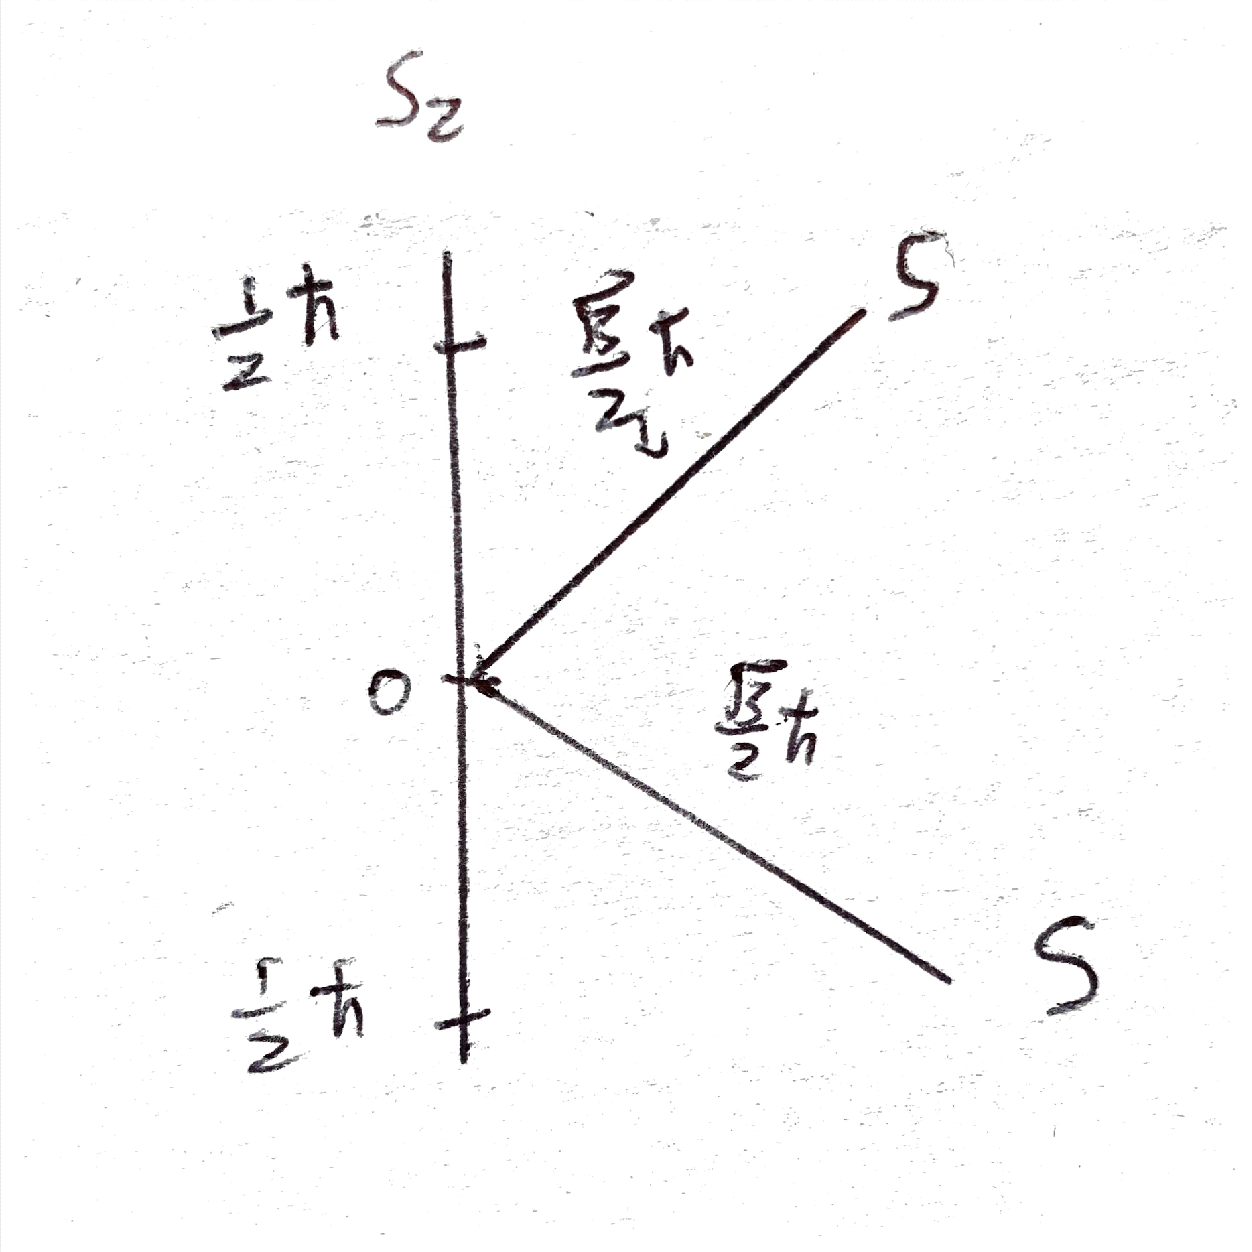
\includegraphics[width=0.3\textwidth]{q1.pdf}
\end{solution}

\question{There exist subatomic particles with spin magnitudes different from that of the electron. However, in all cases they obey the same rules: The magnitude of $\vec{S}$ is $\sqrt{s(s+1)}\hbar$, where  $s$ is a fixed number, integer or half-integer; and the possible values of $S_z$ are $M_s\hbar$, where $m_s$ has the values $s,s-1,\dots,-s$.}

\begin{parts}
\part{For a particle with $s=1$, how many different values of $S_z$ are there, and what are they?}
\part{Draw a vector model diagram similar to Fig 8.14 showing the possible orientations of $\vec{S}$.}
\part{What is the minimum possible angle between $\vec{S}$ and the $z$ axis?}
\end{parts}

\begin{solution}
	There are 3 values, which are $-\hbar,0,\hbar$. The minimum angle is where $m_s = \pm1$. Solving for $\vec{S}$,
	$$\vec{S} = \sqrt{s(s+1)}\hbar = \sqrt{2}\hbar$$
	Then the angle is
	$$\theta = \arccos\left(\frac{S_z}{S}\right) = \arccos\left(\frac{\pm1}{\sqrt{2}}\right) = \frac{\pi}{4}$$
	where the other solution $\frac{3\pi}{4}$ is ignored similarly.
	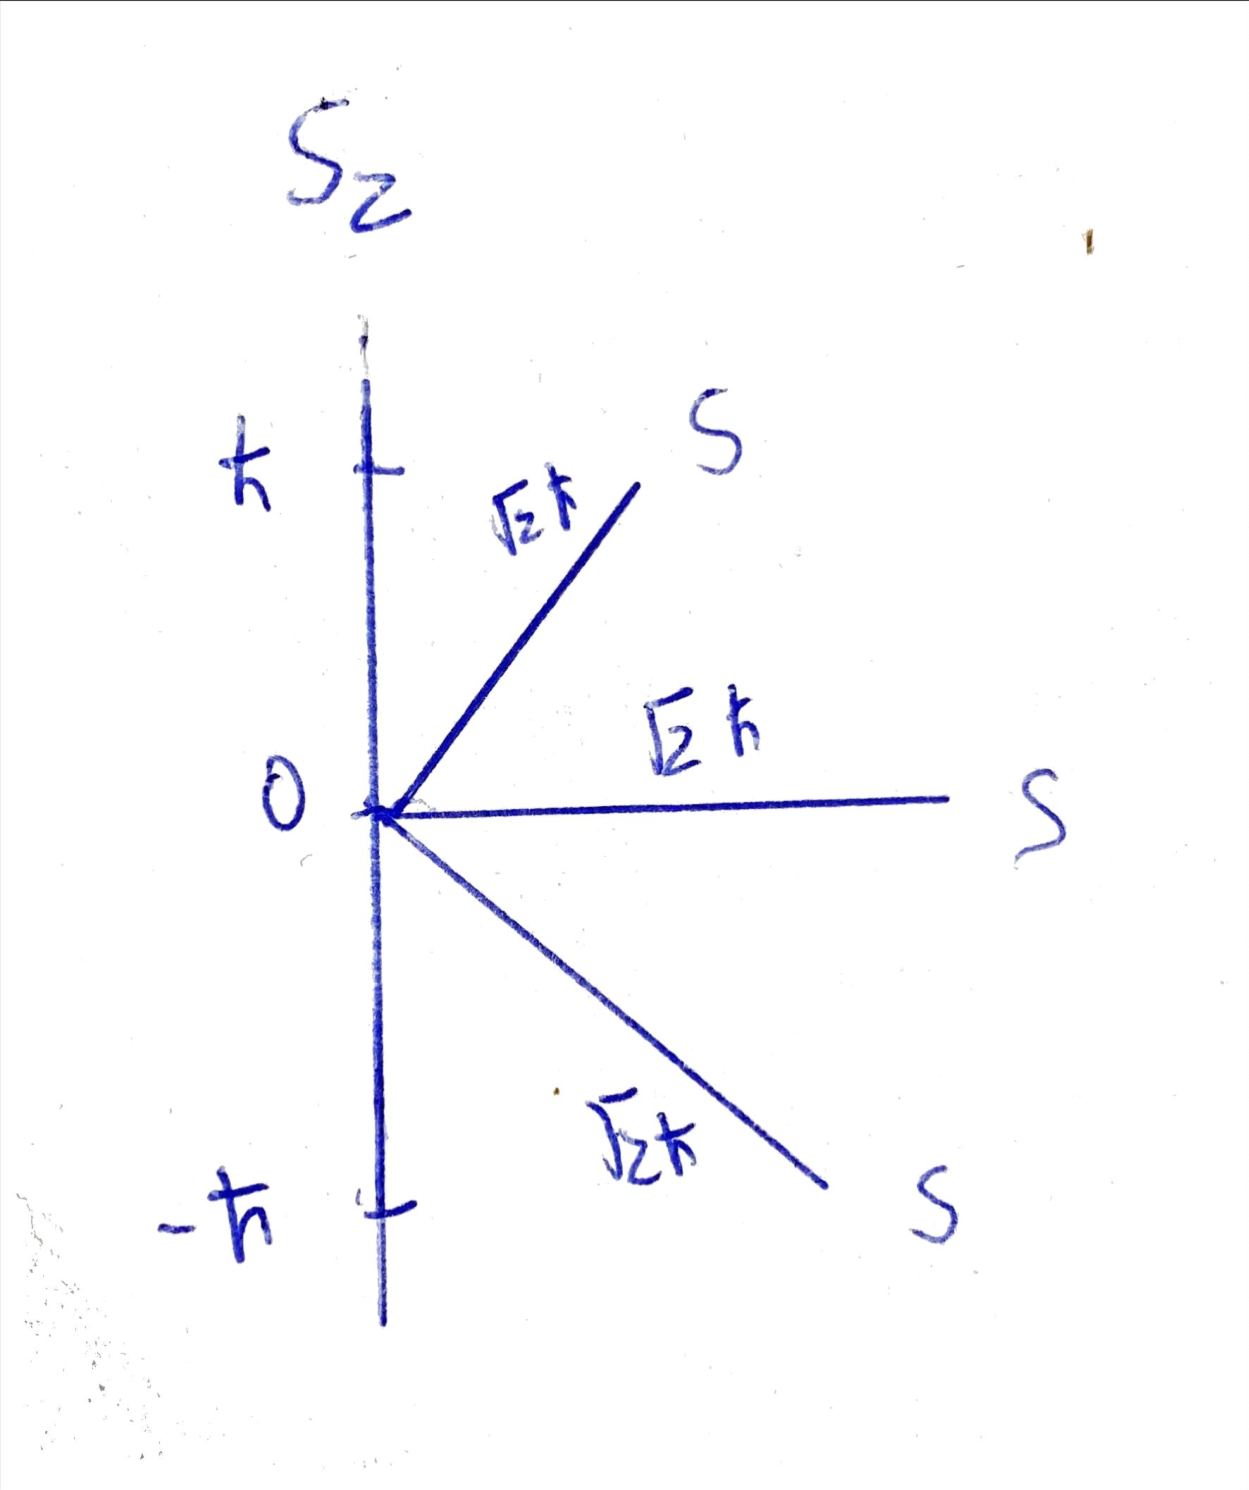
\includegraphics[width=0.3\textwidth]{q2.pdf}
\end{solution}

\question{Make a table showing the values of the four quantum numbers $n,l,m,m_s$ and the energies for each of the 10 lowest-lying quantum states (not energy levels) of a hydrogen atom.}

\begin{solution}
	\begin{center}
	\begin{tabular}{|c|c|c|c||c|}
	\hline
	$n$ & $l$ & $m$ & $m_s$ & $E$ \\
	\hline\hline
	1 & 0 & 0 & $\frac{1}{2}$ & -13.6 \\
	\hline
	1 & 0 & 0 & $-\frac{1}{2}$ & -13.6 \\
	\hline
	2 & 0 & 0 & $\frac{1}{2}$ & -3.4 \\
	\hline
	2 & 0 & 0 & $-\frac{1}{2}$ & -3.4 \\
	\hline
	2 & 1 & -1 & $\frac{1}{2}$ & -3.4 \\
	\hline
	2 & 1 & -1 & $-\frac{1}{2}$ & -3.4 \\
	\hline
	2 & 1 & 0 & $\frac{1}{2}$ & -3.4 \\
	\hline
	2 & 1 & 0 & $-\frac{1}{2}$ & -3.4 \\
	\hline
	2 & 1 & 1 & $\frac{1}{2}$ & -3.4 \\
	\hline
	2 & 1 & 1 & $-\frac{1}{2}$ & -3.4 \\
	\hline
	\end{tabular}
	\end{center}
\end{solution}

\question{We have said that a classical picture of the electron as a spinning ball of matter is unsatisfactory. To illustrate this, consider the following: Modern measurements show that the electron's radius is certainly less than $10^{-18}\unit{m}$. Write an expression for the angular momentum of a uniform spinning ball of mass $m_e$, radius $r$, and equatorial speed $v$. By equating this to the observed spin $\frac{\sqrt{3}\hbar}{2}$, find the minimum possible value of $v$. What is $\frac{v}{c}$?}

\begin{solution}
	$$\vec{L} = \vec{r}\times\vec{p}$$
	so
	$$L = m_evr < 9.11\times10^{-31}\times10^{-18}v$$
	Dividing and rearranging,
	$$v > 1.00\times10^{14}$$
	which is greater than lightspeed.
	$$\frac{v}{c} = 334368 > 1$$
\end{solution}

\question{A current of $0.4\unit{A}$ flows around a single circular loop of radius $1\unit{cm}$. 
}

\begin{parts}
\part{What is the resulting magnetic moment, $\mu$?}
\part{If the loop is placed in a magnetic field $B=1.5\unit{T}$, with $\vec{\mu}$ perpendicular to $\vec{B}$, what is the torque on the loop?}
\part{What is the difference in energy between the cases that $\vec{\mu}$ is parallel to $\vec{B}$ and antiparallel?}
\end{parts}

\begin{solution}
	$$\mu = iA = 4\pi\times10^{-5}$$
	$$\Gamma = \mu B = 6\pi\times10^{-5}$$
	The difference in energy ranges from $0$ to $6\pi\times10^{-5}$, as torque, which is a cross product, vanishes when $\vec{\mu}$ is parallel to $\vec{B}$.
\end{solution}

\question{A typical atomic magnetic moment is of order $10^{-23}\unit{A.m^2}$. Assuming that this is the result of a current $i$ circulating around a single circular loop of radius $0.1\unit{nm}$ (a typical atomic radius), how big is $i$?}

\begin{solution}
	\begin{align*}
		\mu &= iA \\
		10^{-23} &= i\pi\times10^{-20} \\
		i &= \frac{1}{1000\pi} \\
		  &= 3.18 \times 10^{-4}
	\end{align*}
\end{solution}

\question{A helium atom is in an energy level with one electron occupying an $s$ state ($l=0$) and the other an $f$ state $(l=3)$. The two electron spins are antiparallel so that the spin magnetic moments cancel. The atom is placed in a magnetic field $B = 0.8\unit{T}$.}

\begin{parts}
\part{Sketch the resulting splitting of the original energy level.}
\part{What is the energy difference between adjacent levels of the resulting multiplet?}
\end{parts}

\begin{solution}
	$$\Delta E = m\mu_BB = 5.79\times10^{-5}\times 0.8m = 4.63\times10^{-5}m$$
	The energy difference between adjacent levels is thus $4.63\times10^{-5}\unit{eV}$. \\
	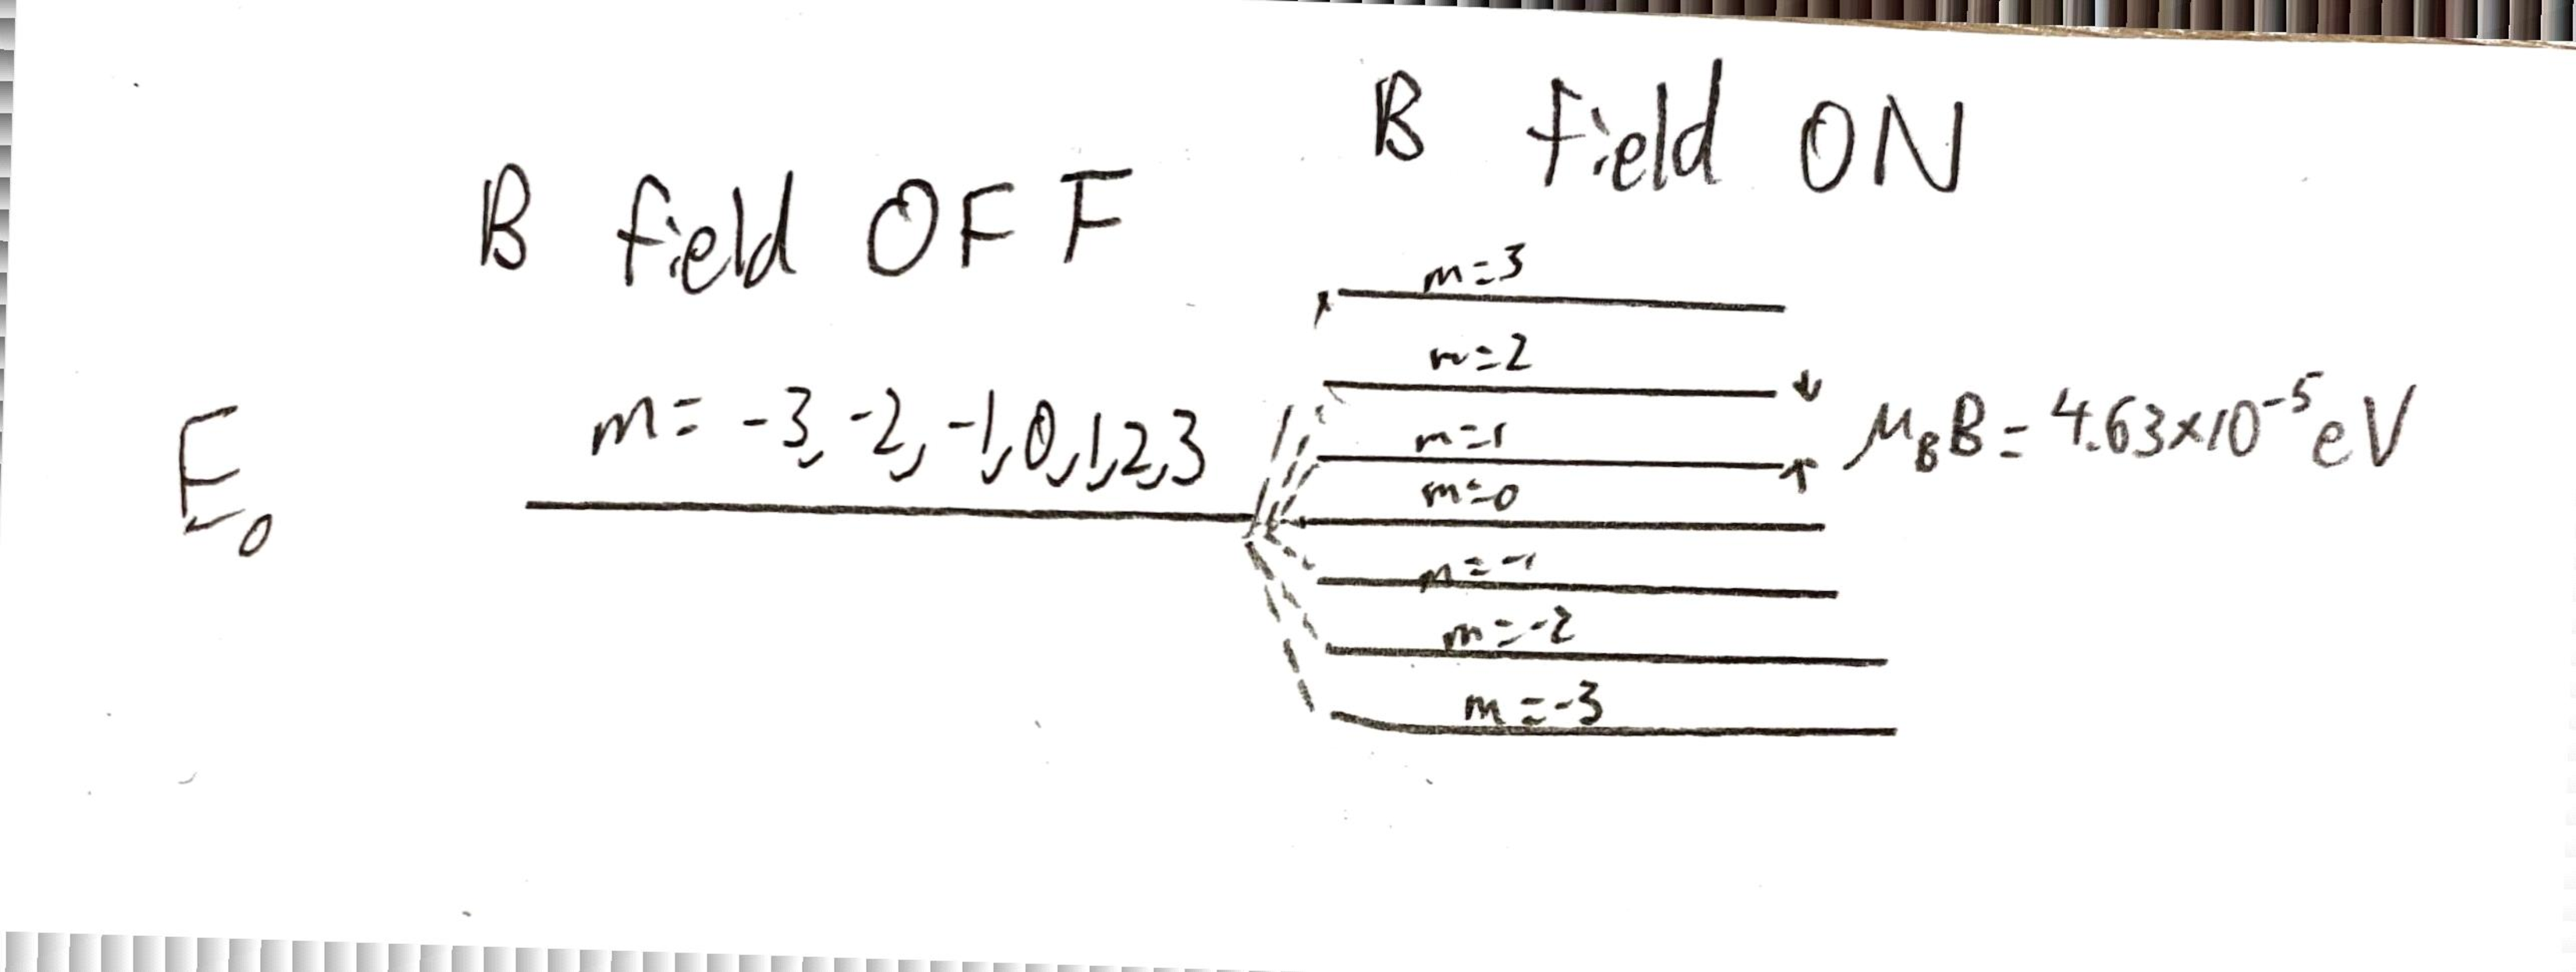
\includegraphics[width=0.7\textwidth]{q-3.pdf}
\end{solution}

\question{Consider two levels of the helium atom in both of with the spins are antiparallel and one electron is in an $s$ state ($(l=0)$. In the higher level the second electron occupies a $d$ state $(l=2)$, and in the lower level it occupies a $p$ state $(l=1)$.}

\begin{parts}
\part{Sketch the splitting of both levels resulting from a magnetic field along the $z$ axis.}
\part{Imagine a transition from one of the $d$ states, with $L_z=m_i\hbar$, to one of the $p$ states, with $L_z=m_f\hbar$. Since $m_i$ can be $2,1,0,-1$, or $-2$ and $m_f$ can be $1,0$, or $-1$, there are $5\times3$ or 15 distinct conceivable transitions. How many different photon energies would these 15 transitions produce?}
\part{Not all of these 15 transitions occur. In fact, it is found that the only transitions observed are those for which
	$$(m_f-m_i) \in \{1,0,-1\}$$
Prove that because of the restriction, there are only three distinct photon energies produced in all possible transitions.}
\end{parts}

\begin{solution}
	$$E = E_d - E_p = E_{dp} + \Delta E_d - \Delta E_p = E_{dp} + (m_i-m_f) \mu_BB$$
	where $E_{dp}$ is the energy without splitting. Then the number of possible energies is the number of possible values of $(m_i-m_f)$. This ranges from -3 to 3, so there are 7 possible energies. Under the restriction, there are only three distinct energies. \\
	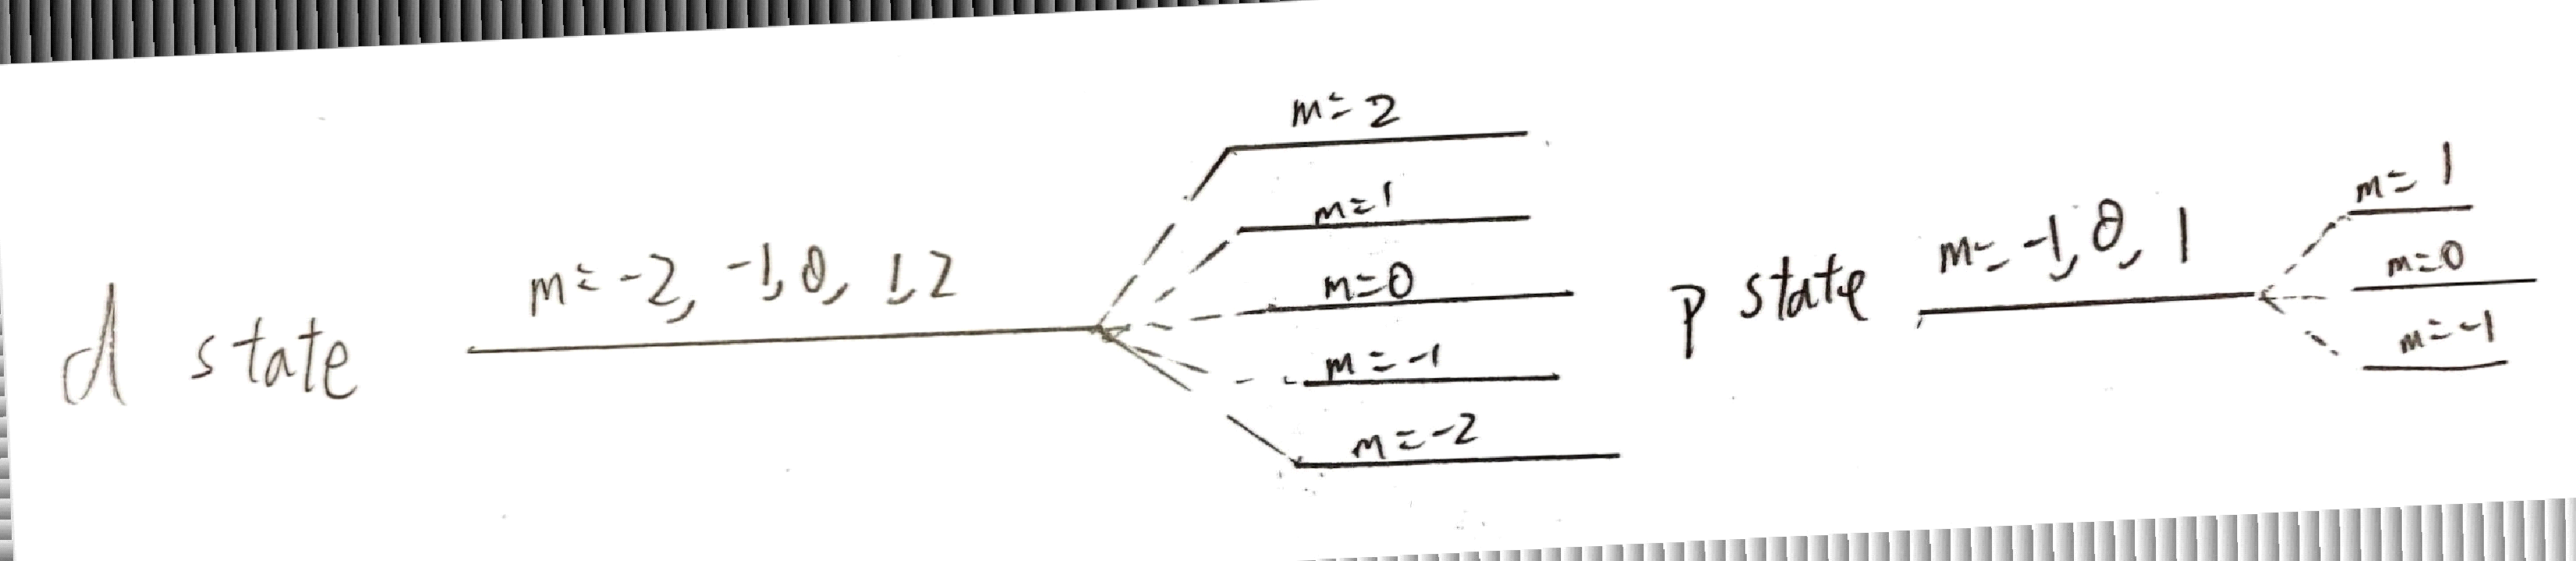
\includegraphics[width=0.7\textwidth]{q-2.pdf}
\end{solution}

\question{Consider a hydrogen atom in its ground leve, placed in a magnetic field of $0.7\unit{T}$ along the $z$ axis.}

\begin{parts}
\part{What is the energy difference between the spin-up and spin-down states?}
\part{An experimenter wants to excite the atom from the lower to the upper state by sending in photons of the appropriate energy. What energy is this? What is the wavelength? What kind of radiation is this? (Visible? UV? etc.)}
\end{parts}

\begin{solution}
	The energy difference is given by
	$$2\mu_BB = 2\times5.75\times10^{-5}\times0.7 = 8.05\times10^{-5}$$
	The wavelength is then
	$$\frac{hc}{\lambda} = 8.05\times10^{-5} \Rightarrow \lambda = 0.0154\unit{m}$$
	which is a microwave.
\end{solution}
\end{questions}
\end{document}
